\documentclass[12pt,aspectratio=169]{beamer}

\usetheme[version=2019]{iiasa}

\usepackage{biblatex}
\addbibresource{all.bib}

\usepackage{minted}

\title{Collaborative development of academic software}
\institute{IIASA Energy, Climate, and Environment program}

% \date{MESSAGE workshop — Friday, 4 October 2019}
% \date{MESSAGE workshop — Friday, 12 June 2020}
% \date{MESSAGE workshop — Thursday, 10 September 2020}
% \date{Tutorial — Friday, 5 February 2021}
% \date{MESSAGE workshop — Thursday, 10 June 2021}
% \date{MESSAGE workshop — Friday, 10 June 2022}
\date{MESSAGE workshop — Monday, 12 June 2023}

\author{\texorpdfstring{Paul Natsuo Kishimoto \scriptsize\newline
  \href{mailto:paul.kishimoto@iiasa.ac.at}%
       {\ttfamily <paul.kishimoto@iiasa.ac.at>}}%
  {Paul Natsuo Kishimoto <paul.kishimoto@iiasa.ac.at>}}

\begin{document}

\maketitle

\begin{frame}{Colophon}

  These slides have been used for:
  \begin{itemize}
    \item MESSAGEix training \& capacity-building workshops given by the IIASA Energy Program on \structure{2020-06-12}, \structure{2020-09-10}, \structure{2021-06-10}, \structure{2022-06-10}, and \structure{2023-06-12}.

    \item A tutorial on \structure{2021-02-05} with participants from the International Transport Forum at the OECD and IIASA/ECE.
  \end{itemize}

  \medskip
  A different subset of the slides was used on each occasion.

  \medskip
  LaTeX source, copyright, \& license available at \url{https://github.com/khaeru/doc/}.

\end{frame}

% \begin{frame}<0>[noframenumbering]  % on 2021-02-05
\begin{frame}  % other uses
  \frametitle{Review}

  Previously:
  \begin{description}
    \item [Session I.] MESSAGEix modeling framework \& software stack.
    \item [Session II/III.] Energy systems modeling in MESSAGEix.
  \end{description}

  \bigskip
  Today:
  \begin{description}
    \item [$N \approx 20$'] Collaborative research using models.


    \item [$(115 - 20) / 2$'] Collaborative research using models.

          (Hint: it's software development!)

          \structure{Outcome:} you understand core concepts and terms, as a basis for continued learning \& skill development.

    \item [5'] Break.

    \item [$(115 - 20) / 2$'] Reporting and post-processing.

          The \texttt{westeros\_report.ipynb} tutorial.
  \end{description}

\end{frame}


\begin{frame}{Syllabus}

  \begin{enumerate}
    \item [C.] MESSAGE-GLOBIOM research.
          \begin{enumerate}
            \item [1.] \textbf{Validity \& reproducibility (r13y) for modeling \& scenario research.} Internal vs.\ external validity. Perspectives on models. Validity vs.\ r13y. Modeling practices for r13y.
          \end{enumerate}

    \item [D.] MESSAGEix development.
          \begin{enumerate}
            \item [2.] \textbf{Version control using {\ttfamily git} \& GitHub.} Version control in general. \texttt{git} and concepts: commit, branch, diff, tag, repo, merge, fetch/pull/push.
            \item [3.] \textbf{Collaborative development using GitHub.} Collaboration decisions. GitHub flow. Issue, pull request, milestone, project. Examples \& demo.
            \item [4.] \textbf{Test-driven development.} Purpose. Types of tests. Test coverage. \texttt{pytest} intro.
            \item [5.] \textbf{Continuous integration.} Purpose. GitHub Actions, RTD, Codecov, Stickler.
          \end{enumerate}

  \end{enumerate}

  % → \href{https://iiasahub.sharepoint.com/:w:/s/ene/MESSAGEix/EQEFlE-gGNNMpHXgYP-MJmABuoYVPDMqPbcSnjGq4QZ0ZQ?e=LCBJah}{Full syllabus} (IIASA/ENE SharePoint). Not covered today: C2–3, D1.

\end{frame}

\begin{frame}{Outline}
  \tableofcontents[hideallsubsections]
\end{frame}

\begin{frame}{Motivation}
  \framesubtitle{Thinking about costs}

  We have finite resources (time, energy, money) with which to conduct research.
  Tasks related to model development should use those resources efficiently.

  \bigskip
  \structure{Search \& information costs}

  \begin{itemize}
    \item How do I run the model? What does this line of code do?
    \item What about student/visitor X, who did Y two years ago—where is that version?
    \item What version of the model did I use to produce the results for paper X, which has been under review for 6 months?
  \end{itemize}

\end{frame}

\begin{frame}{Motivation}
  \structure{Policing \& enforcement costs}

  \begin{itemize}
    \item Who broke the model so Policy Z no longer has a feasible solution?
    \item When did our reference forecast start doing this weird thing in region $r$ \& sector $g$?
    \item What is our definitive ‘reference’ projection?
          Why does it differ between these two papers?
    \item Who changed this parameter \& caused this reviewer to yell at me?
  \end{itemize}

  \bigskip
  \structure{Recovery/disruption costs}

  The \emph{bus factor} or \emph{truck number}—“How many people would need to be hit by a truck, tomorrow, for us to suffer a serious setback in continuity/loss of work?”

\end{frame}

\section{C1. Reproducible research}
\begin{frame}{C1. Reproducible research}
  \tableofcontents[hideothersubsections]
\end{frame}

\subsection{Internal vs.\ external validity}
\begin{frame}{Internal vs.\ external validity}
\framesubtitle{Concerns for scientific modeling \& scenario research}

\structure{Internal validity.} Research is free of errors:

\begin{itemize}
  \item Correctly implements theory w/o conceptual errors.
  \item Confounding variables addressed to identify relationships between independent and dependent variables.
  \item Alternative hypotheses can be rejected.
\end{itemize}

\bigskip
\structure{External validity.} Research is generalizable to other conditions:

\begin{itemize}
  \item Research can be replicated or reproduced in a different context.
  \item Research is robust to differences between the study context and other contexts to which conclusions are applied.
  \item Research is robust to plausible alternatives to key assumptions.
\end{itemize}

\end{frame}


\subsection{What is a model?}
\begin{frame}[allowframebreaks]{What is a model?}
\framesubtitle{Three perspectives and resulting insights}

A \structure{knowledge object} that embodies or represents a theory or understanding of some real-world phenomenon.

\medskip
\begin{itemize}
  \item Theories often causal.
  \item Relationships expressed quantatively: equations connecting variables representing concepts measured in certain, systematic ways.
  \item In large-scale integrated assessment, systematized concepts often aggregate: GDP, country, sector.
\end{itemize}

\framebreak
A \structure{scientific instrument}\footcite{omalley-2019} that is used to perform experiments: “What would be the outcome (effect on quantity $Y$) if $X$ were changed from $x_1$ to $x_2$?”

\medskip
\begin{itemize}
  \item Another instrument: the Large Hadron Collider (LHC).
    \begin{itemize}
      \item EUR 7.5 billion budget; labour from many specialized roles.
      \item Components for preparing the experiment, running it, measuring outcomes are carefully designed, constructed, tested.
    \end{itemize}
  \item Instruments require meticulous attention to detail.
  \item Description of methods includes description of instruments, so the experiment can be reproduced.
\end{itemize}

\framebreak
A \structure{software project} in which people in organizations create code that is run on computer systems.

\medskip
\begin{itemize}
  \item All software has bugs; all organizations have politics.
  \item Software is constantly evolving and never complete.
  \item Tendency to overinvest time in new code vis-à-vis quality \& docs.
  \item “Technical debt”: code grows stale over time.
\end{itemize}

\med
\structure{\bfseries But!} good software development practices exist, and are widely used to ensure that software meets needs.

\end{frame}


\begin{frame}{Validity and reproducibility (r13y)}

  Since the model is not the real world, implications drawn from modeling results must be externally valid.
  Specific threats, as forms of uncertainty:

  \begin{description}
    \item [Structural.] Is the theory a correct description of the phenomena?

          → Responses: alternate model formulations.

    \item [Measurement] uncertainty of input data and parameters.

          → Sensitivity analyses, large ($>10^3$) ensembles of model runs.

    \item [Epistemic] uncertainty in conditions (e.g. future policy) that are unknowable, or whereof uncertainty cannot be quantified.

          → Alternate scenarios.
  \end{description}

  All require a \structure{quality} instrument that can be \structure{reused in an easy, automated manner}, giving the \structure{same results every time}—a \structure{\bfseries reproducible} model.
\end{frame}

\subsection{Modeling practice for validity \& reproducibility}
\begin{frame}{Modeling practice for validity \& r13y}

  A collection of mutually-reinforcing practices:
  \begin{itemize} \small
    \item Version control.
    \item Collaborative development and documentation.
    \item Making software and data free and open in permanent archives.
    \item Internal \& external peer review of modeling software.
    \item Manual or automated (continuous) testing.
    \item Organization and incentives to do the above.
  \end{itemize}

  \bigskip
  Adopting best practices helps immensely, but is \structure{only part of} ensuring validity and reproducibility.
  Other research tactics (e.g. careful \emph{ex post} checks) also help—but they can be costly.

\end{frame}

\begin{frame}[plain]
  \centering
  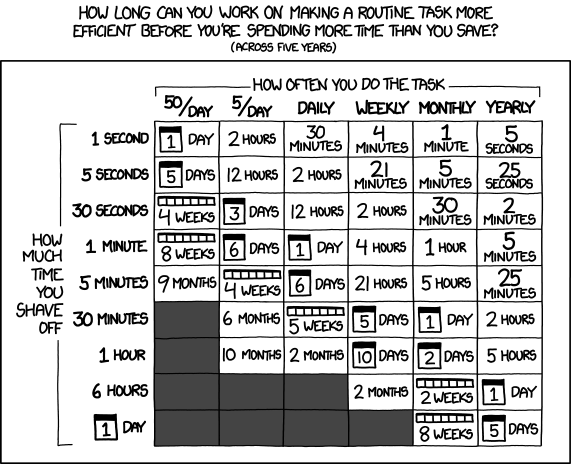
\includegraphics[height=\paperheight]{xkcd_1205.png}
\end{frame}

\begin{frame}{Wrapping up: costs again}

  R13y in principle ≠ a habit of frequent reproduction.

  If costs of reproduction are too high, people have little incentive to…
  \begin{itemize}
    \item often or ever try to reproduce results.

    \item identify, disclose, and correct internal \emph{invalidity} (i.e. modeling errors).
  \end{itemize}

  \bigskip
  When research methods are \structure{tacit knowledge} rather than embodied in software, personnel changes make the cost of reproduction go up.

  \begin{itemize}
    \item Personnel changes are frequent in academia.
  \end{itemize}

  \bigskip
  \structure{\bfseries Conclusion} → improve modeling practices in pursuit of reproducibility.

\end{frame}

\subsection{Further reading}
\begin{frame}{Further reading}
  \begin{itemize}
    \small
    \item L. Barba group @ GWU SEAS: \href{http://lorenabarba.com/blog/barbagroup-reproducibility-syllabus/}{r13y syllabus} w/readings on research group website; \href{http://science.sciencemag.org/content/354/6308/142}{``The Hard Road to Reproducibility''} in \emph{Science}.
    \item Max Planck Institute for Meteorology \href{http://mpimet.mpg.de/en/science/publications/good-scientific-practice.html}{``Good scientific practice''} policy, rules, forms.
    \item Irving (2016), \href{http://journals.ametsoc.org/doi/abs/10.1175/BAMS-D-15-00010.1}{``A Minimum Standard for Publishing Computational Results in the Weather and Climate Sciences''} in \emph{Bulletin of the AMS}.
    \item Christensen \& Miguel (2016), \href{http:/dx.doi.org/10.3386/w22989}{``Transparency, Reproducibility, and the Credibility of Economics Research''} forthcoming in \emph{JEL} — UC Berkeley Econ.
    \item Nick Barnes: \href{https://www.nature.com/news/2010/101013/full/467753a.html}{``Publish your computer code: it is good enough''} in \emph{Nature News} — Climate Code Foundation.
    \item \href{http://ropensci.github.io/reproducibility-guide/sections/references/}{45+ more peer-reviewed articles} and other resources.
  \end{itemize}
\end{frame}

\section*{D. MESSAGEix development}
\begin{frame}{Unit D: MESSAGEix development}

  This section presents an overview of the processes and tools used in development of the MESSAGE\emph{ix} framework, ixmp, and the MESSAGEix-GLOBIOM model family of IIASA's Energy Program

  \medskip
  References:
  \begin{itemize}
    \item \url{https://docs.messageix.org} → “Contributing to development”

    \item Existing content on GitHub, e.g. repositories
          \href{https://github.com/iiasa/message_ix}{\ttfamily iiasa/message\_ix},
          \href{https://github.com/iiasa/ixmp}{\ttfamily iiasa/ixmp}.
  \end{itemize}

  \medskip
  However, the concepts, tools, and processes are generalizable to any other model implemented as software.

  % \begin{itemize}
  %   \item \url{https://docs.messageix.org} \\
  %     → \texttt{v: main} (bottom-left) → “Contributing to MESSAGEix development”
  %
  %   \item MESSAGEix SharePoint site and linked documents:
  %     \url{https://iiasahub.sharepoint.com/sites/ene/MESSAGEix/}
  %
  %   \item Existing content on GitHub, e.g. repositories
  %     \href{https://github.com/iiasa/message_ix}{\ttfamily iiasa/message\_ix},
  %     \href{https://github.com/iiasa/ixmp}{\ttfamily iiasa/ixmp},
  %     \href{https://github.com/iiasa/message_data}{\ttfamily iiasa/message\_data} (private)
  % \end{itemize}
  %
  % \medskip
  % As we go through lessons D2–D5, ask:
  % \begin{itemize}
  %   \item is the Energy Program's \emph{specific} practice of software development described/obvious from these resources?
  %   \item is it clear \emph{why} we do things in one way, but not another?
  % \end{itemize}
  %
  % \medskip
  % \centering \Large
  % \alert{No?} → please speak up!

\end{frame}


\section{D2. Version control using git \& GitHub}
\begin{frame}{D2. Version control using git \& GitHub}
  \tableofcontents[hideothersubsections]
\end{frame}

\subsection{Version control systems}
\begin{frame}{Version control systems}

  \structure{Version control} is the management of changes to documents, computer programs and other collections of information.

  \begin{itemize}
    \item Changes or states usually identified by a number or letter code.
    \item Each revision associated with a \emph{timestamp} and \emph{author}.
    \item Revisions can be \emph{compared}, \emph{restored}, and \emph{combined}.
  \end{itemize}

  \bigskip
  \structure{Version control systems} (VCS, “revision control systems”, other names) are software that tracks and provide control over revisions.

  \begin{itemize}
    \item Automate repetitive, boring processes.
          \begin{itemize}
            \item These could be (often are!) done manually.
            \item But, because they are monotonous, mistakes are likely.
          \end{itemize}
    \item Manage the chronological and sequential relationship between revisions.
  \end{itemize}

\end{frame}

\subsection{\texttt{git} concepts}
\begin{frame}{\texttt{git}: a VCS}

  Several different VCS available.
  Some tools (e.g. Dropbox; MS Office “track changes”) provides a subset of VCS-like features…but not suitable for models and scientific code.

  \bigskip
  We use \structure{\ttfamily git} because it is popular, thus well-supported.
  \begin{itemize}
    \item A command-line (CLI) tool.
    \item Many GUI applications wrap around the CLI.

          E.g.
          \href{https://desktop.github.com/}{GitHub Desktop},
          \href{https://vscode.github.com/}{Visual Studio Code},
          \href{https://www.gitkraken.com/}{GitKraken}.
  \end{itemize}

  \bigskip
  \structure{This lesson:} a quick tour of key \texttt{git} concepts.
  \begin{itemize}
    \item \emph{Many} more resources available online—search and find some;
          identify the ones most helpful to you.
    \item Here we use diagrams from the \href{https://git-scm.com/book/en/v2/Getting-Started-What-is-Git\%3F}{Git Book} (available in 19+ languages).
  \end{itemize}
\end{frame}

\begin{frame}[fragile]{\texttt{git} concepts: commit} \large
  A single version of a set of files arranged in directories.

  \bigskip
  \begin{itemize}
    \item Author, timestamp, files (‘blobs’), description.
    \item ID or ‘hash’ e.g. \texttt{3f2ca4130cab262cfac62c5a98dd2ebdeb424dc5}.
          \begin{itemize}
            \item We abbreviate with the first few characters: \texttt{3f2ca413}
          \end{itemize}
    \item Hash of a previous (‘parent’) commit.
    \item ‘Snapshots’ of each file.
  \end{itemize}
\end{frame}

\begin{frame}[plain]
  \centering 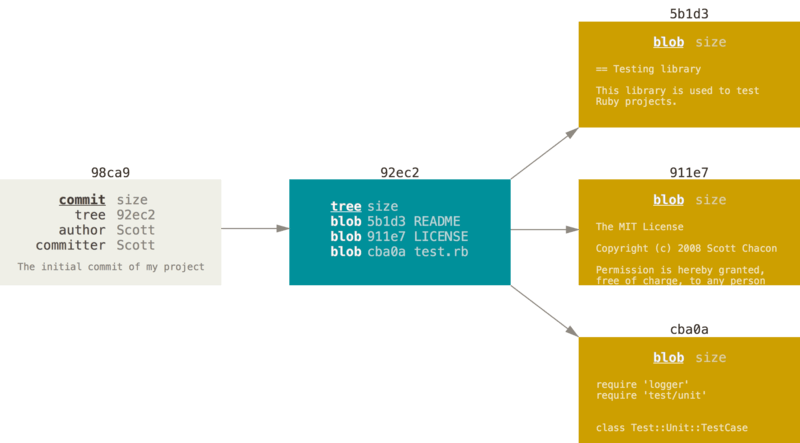
\includegraphics[height=0.8\textheight]{commit-and-tree.png}
\end{frame}

\begin{frame}{\texttt{git}: branch} \large
  A name for a particular commit \emph{and} its ancestors:

  \centering
  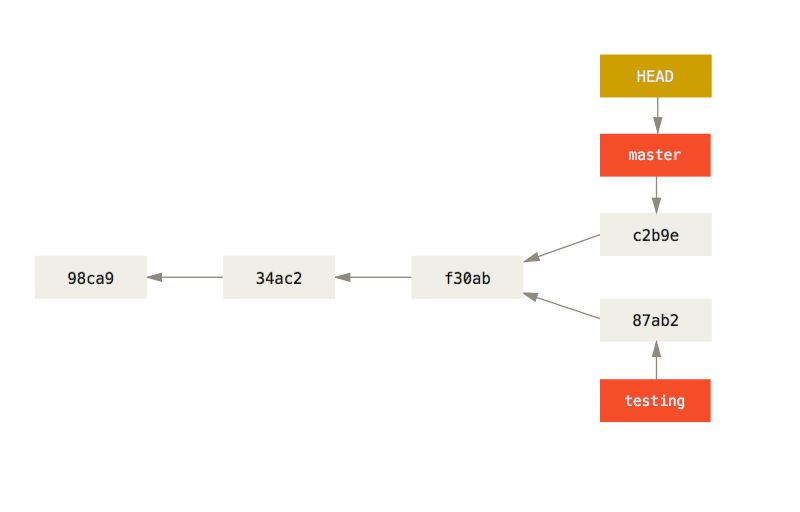
\includegraphics[height=0.9\textheight]{advance-master.png}
\end{frame}

\begin{frame}{\texttt{git}: branch}
  Commits may share the same snapshot of a file → storage efficiency.

  \includegraphics[width=\textwidth]{snapshots.png}
\end{frame}

\begin{frame}[fragile]{\texttt{git} concepts: diff}
  Used to express changes between two snapshots of a single file:

  \bigskip
  \begin{columns}[t]
    \column{0.3\paperwidth}
    Original file:

    \begin{minted}[bgcolor=gray!25]{text}
Shopping List

* Apples
* Oranges
* Salt
* Pepper
\end{minted}

    \column{0.3\paperwidth}
    Modified file:

    \begin{minted}[bgcolor=gray!25]{text}
Shopping List
for Friday

* Apples
* Oranges (1 dozen)
* Salt
\end{minted}

    \column{0.3\paperwidth}
    Changes

    \begin{minted}[bgcolor=gray!25]{diff}
 Shopping List
+for Friday

 * Apples
-* Oranges
+* Oranges (1 dozen)
 * Salt
-* Pepper
\end{minted}

  \end{columns}

  \texttt{git} doesn't store these internally, but understands \& generates them.
\end{frame}

\begin{frame}{\texttt{git}: tag} \Large
  A name applied to a certain commit.

  \bigskip
  A \emph{branch} can be extended by adding more commits to its head.

  A \emph{tag} always stays in the same place.
\end{frame}

\begin{frame}{\texttt{git}: repository (‘repo’)}
  {\Large \centering A collection of commits, snapshots, and tags.}

  \bigskip
  \begin{itemize}
    \item Stored as files in a directory, 100\% self-contained.
    \item Usually, within a \texttt{.git} hidden directory in the \structure{working tree}, i.e. a folder.
  \end{itemize}
\end{frame}

\begin{frame}{\texttt{git}: merge} \Large
  Combines two commits from different branches.

  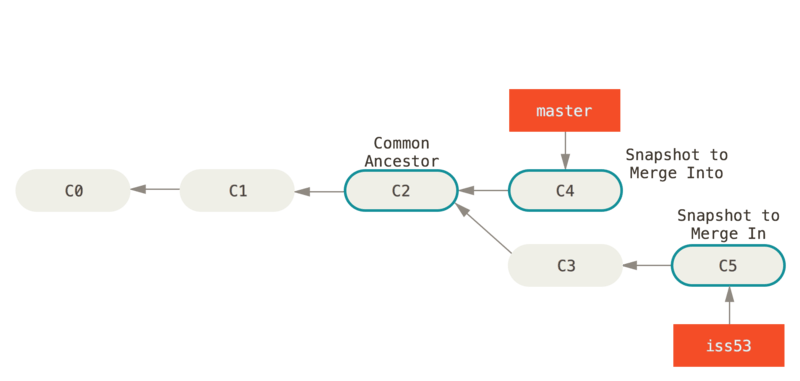
\includegraphics[width=\textwidth]{basic-merging-1.png}
\end{frame}

\begin{frame}{\texttt{git}: merge} \Large
  Creates a new commit.
  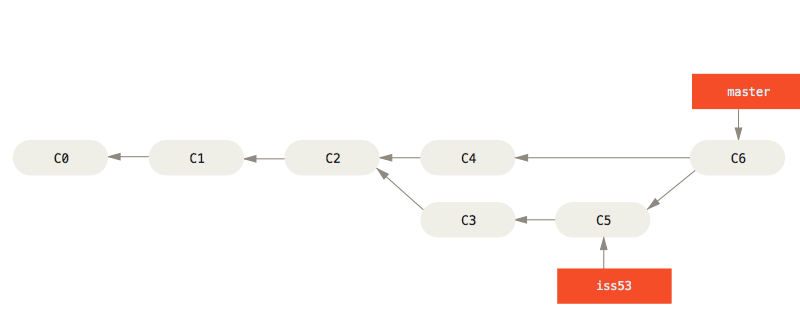
\includegraphics[width=\textwidth]{basic-merging-2.png}
\end{frame}

\begin{frame}{\texttt{git}: merge} \large
  \texttt{git merge} \structure{automatically} handles many tasks.

  \bigskip
  For example, changes to the same file:

  \begin{itemize}
    \item \texttt{branch-a} has a commit that modified \texttt{file.txt} near the top.
    \item \texttt{branch-b} has a commit that modified \texttt{file.txt} near the bottom.
    \item \texttt{git} applies \emph{both} changes because they are non-overlapping, producing a combined \texttt{file.txt}
  \end{itemize}
\end{frame}

\begin{frame}[fragile]{\texttt{git}: merge}
  \begin{columns}[t]
    \column{0.3\paperwidth}
    Branch A changes:

    \begin{minted}[bgcolor=gray!25]{diff}
Shopping List

 * Apples
-* Oranges
+* Oranges (1 dozen)
 * Salt
 * Pepper
\end{minted}

    \column{0.3\paperwidth}
    Branch B changes:

    \begin{minted}[bgcolor=gray!25]{diff}
Shopping List
+for Friday

 * Apples
 * Oranges
 * Salt
-* Pepper
\end{minted}

    \column{0.3\paperwidth}
    Combined changes:

    \begin{minted}[bgcolor=gray!25]{diff}
 Shopping List
+for Friday

 * Apples
-* Oranges
+* Oranges (1 dozen)
 * Salt
-* Pepper
\end{minted}

  \end{columns}

  → keep files \& directories neatly organized.
\end{frame}

\begin{frame}{\texttt{git}: fetch/pull/push}
  \texttt{git} can \emph{move commits} between \emph{two} repos in different places:
  \begin{itemize}
    \item Two folders/directories on the same computer.
    \item Two computers: yours vs. a colleague's, or a server online.
  \end{itemize}

  The other repo is called a \structure{remote}. \texttt{git} helps you:
  \begin{itemize}
    \item Name and track multiple remotes related to the current repo.
    \item Associate a local branch with one branch on one remote.
  \end{itemize}

  \medskip
  Operations
  \begin{itemize}
    \item \structure{fetch}: copy commits, branches, tags from a remote repo to yours.
    \item \structure{pull}: does three things
          \begin{enumerate}
            \item Fetch a remote repo.
            \item \emph{Add} new commits from the remote repo onto associated local branch.
            \item \structure{\emph{Fast-forward}} the pointer to the head of the local branch.
          \end{enumerate}

    \item \structure{push}: pull, but in the opposite direction.
  \end{itemize}

\end{frame}

\begin{frame}{Another visualization}
  \begin{columns}[T]
    \column{0.2\textwidth}
    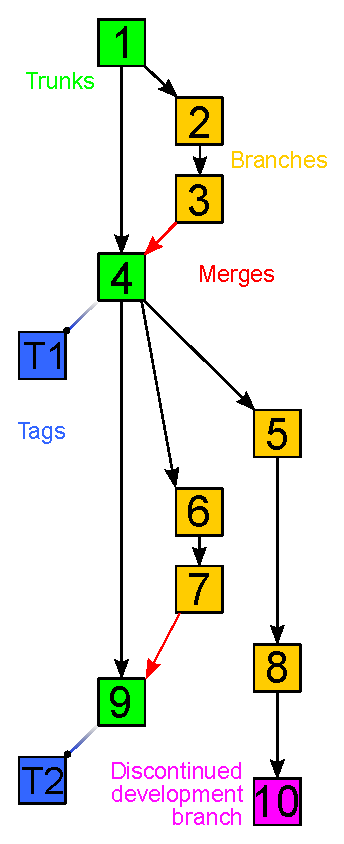
\includegraphics[height=0.8\textheight]{Revision_controlled_project_visualization-2010-24-02.pdf}

    \column{0.8\textwidth}
    \begin{description}
      \item [1, 2, …, 10] commits.
      \item [2, 3] a branch; work done in parallel.
            Others can get \& use \structure{1} while \structure{2}, \structure{3} are developed.
      \item [4, 9] merge commits.

            The changes made in \structure{2}, \structure{3} (or \structure{6}, \structure{7}) are combined with \structure{1} (or \structure{4}) to produce the new revision \structure{4} (or \structure{9}).
      \item [1, 4, 9] the ‘main’ branch

            \emph{Chosen} by the user to be the authoritative version of the code.
      \item [T1, T2] tags.
    \end{description}

  \end{columns}
\end{frame}

\section{D3. Collaborative development using GitHub}
\begin{frame}{D3. Collaborative development}
  \tableofcontents[hideothersubsections]
\end{frame}

\subsection{General concepts}
\begin{frame}{General concepts}

  VCS like \texttt{git} provide \emph{tools} for managing versions of code.

  \bigskip
  They do not:
  \begin{itemize}
    \item Require collaboration.

          You can use \texttt{git} in a single local repo without an Internet connection.
    \item Require that the files/code \emph{do} anything, or be ‘correct’.
    \item Prescribe \emph{how} or \emph{to what end} we should use them.
  \end{itemize}

  \bigskip
  \structure{Software development} comprises…
  \begin{itemize}
    \item the actions of conceiving, specifying, designing, programming, documenting, testing, and bug fixing…
    \item involved in creating and maintaining software.
  \end{itemize}
\end{frame}

\begin{frame}{General concepts}
  \structure{Collaborative development}: when software development involves 2+ people embedded in 1+ organizations.

  \begin{itemize}
    \item Using a VCS can make this a lot easier, but…
    \item All involved must agree on \emph{how} to use the VCS.
  \end{itemize}

  \bigskip
  To collaborate, we must \emph{communicate} about code:
  \begin{itemize}
    \item “[code] used to do X for me, but now it doesn't.”
    \item “[code] says it will do X, but instead does Y.”
    \item “[Al's code] does X, [Bo's code] does Y, but Jo wants to do both.”
    \item “We fixed Y by making [changes] to [code].”
    \item “I wrote [new code] and I want everyone to use it.”
    \item “You should use [version] instead of [version].”
  \end{itemize}

\end{frame}

\subsection{GitHub}
\begin{frame}{GitHub}

  A (very) popular website.

  \bigskip
  You (\structure{user}) or a group (\structure{organization}) can store \texttt{git} repos on their servers.

  \bigskip
  More importantly, provides many tools for software development tasks (previous slide).
  \begin{itemize}
    \item These are tightly tied to specific \texttt{git} repos, branches, commits, and tags.
    \item They make it easy to use a certain \structure{workflow} of software development.
    \item Understanding and using this workflow is a good starting point for academic teams collaborating on research software.
  \end{itemize}

\end{frame}

\begin{frame}{BUT (!)}

  GitHub's features are only \emph{higher-level tools}, built on \texttt{git}.

  \bigskip
  They \emph{suggest} a certain workflow, but every set of collaborators \structure{must still decide} \emph{whether} and \emph{how} to use the features, and \emph{what} their use means.

  \bigskip
  Some such decisions flagged with \alert{(!)} below.
  For example:

  \begin{itemize}
    \item Alice and Bob both run into problems with Model X.
    \item Bob files a bug report (on GitHub)—but no one does anything.
    \item Alice doesn't use GitHub at all. But, her problem results in a new branch with many commits, lots of discussion, a quick merge into \texttt{main}, and a release—all via GitHub.
  \end{itemize}

  → Why did this happen?

\end{frame}

\subsection{GitHub workflow concepts}
\begin{frame}{GitHub workflow concepts: fork}

  A repo that is created by copying another repo.

  \bigskip
  Example:
  \begin{itemize}
    \item \url{https://github.com/iiasa} —IIASA organization.
    \item \url{https://github.com/iiasa/ixmp} —‘main’ repository for ixmp.
          \begin{itemize}
            \item May be \emph{public} or \emph{private}.
            \item Read, write, admin access can be controlled.
          \end{itemize}
    \item \url{https://github.com/khaeru} —a user's profile.
    \item \url{https://github.com/khaeru/ixmp} ­—user's \structure{fork} of ixmp.
  \end{itemize}

  \bigskip
  Useful for working on changes for private use, or isolating work before it is merged with the main repo.

  Can view all forks from a repo.

\end{frame}


\begin{frame}{GitHub: release}

  { \Large
    A \texttt{git} tag with \structure{title}, \structure{description}, and \structure{associated downloads}.}

  \bigskip
  Example:

  \url{https://github.com/iiasa/ixmp/releases} —all releases of ixmp.

\end{frame}

\begin{frame}{GitHub: issue}
  A discussion about some bug, planned feature, or other issue \alert{(!)} related to a specific repo.

  \bigskip
  Example: \url{https://github.com/iiasa/message_ix/issues/571}

  \bigskip
  \begin{itemize}
    \item Identified by a number: \texttt{iiasa/message\_ix\#571}.
    \item \structure{Title} and \structure{description} from by the user who opened it.
    \item \structure{comments} from others.
    \item Can be \structure{assigned} to a particular user.

          \alert{(!)} the person responsible for fixing/addressing it?
    \item Can be associated with a \structure{label}, \structure{milestone} (later), or \structure{project} (later).
    \item \structure{Status}: open or closed.
          \alert{(!)} Does ‘closed’ mean ‘fixed’?
    \item \url{https://github.com/iiasa/message_ix/issues} —all issues for a repo.

          \hspace{2em} Search \& filter tools.
  \end{itemize}

\end{frame}

\begin{frame}{GitHub: pull request (PR)}
  A request to \texttt{git} merge one branch into another (the ‘base’).

  \bigskip
  Example: \url{https://github.com/iiasa/message_ix/pull/572}

  \bigskip
  \begin{itemize}
    \item Similar to issues: title, description, assignee(s), comments, label, milestone, project.
    \item Status: open, merged, or closed [without merging].
    \item \structure{Reviewer(s)} — similar to assignees, 0+ other users (next slide).
    \item List of commits since the common ancestor.
    \item Collective diff for all changes introduced in the branch.
    \item \structure{Checks} related to continuous integration tools (next lesson).
  \end{itemize}

  \alert{Caution:} a branch named \texttt{iiasa:example} is not the same as
  \texttt{khaeru:example}!

\end{frame}

\begin{frame}{GitHub: PR (continued)}
  Pull requests can \emph{close} a specific issue, e.g. by fixing a bug or adding a desired feature.

  \bigskip
  \structure{Reviewers} are requested, can view the commits and diff.
  \begin{itemize}
    \item Add comments on specific changed lines.
    \item Approve, request changes, or just comment.
  \end{itemize}

  \bigskip
  \alert{(!)} Collaborators must decide \emph{how} to use PRs/reviews:

  \begin{itemize}
    \item Are reviews required? How many?
    \item Who can review the code?
    \item Different reviewers for different parts of code/types of issues or PRs?
    \item Should the code itself contain certain things?
  \end{itemize}

  \smallskip
  \hspace{2em} \url{https://github.com/iiasa/message_ix/pulls} —all PRs for a repo.

\end{frame}

\begin{frame}{GitHub: milestone}

  {\Large A target for collecting issues and pull requests.}

  \bigskip
  Example: \url{https://github.com/iiasa/message_ix/milestone/12?closed=1}

  \begin{itemize}
    \item \structure{Title} and \structure{description}.
    \item \structure{Status}: open or closed.
    \item Can be assigned a \structure{target date}.
    \item \alert{(!)} What happens when the date passes?
    \item \alert{(!)} Is a release created when the milestone is reached?
  \end{itemize}

\end{frame}

\begin{frame}{GitHub: project}

  {\Large \emph{Kanban}-style system for organizing multiple \structure{tasks}.}

  \bigskip
  Example: \url{https://github.com/orgs/iiasa/projects/3}

  \begin{itemize}
    \item \structure{Cards} for tasks that are either text (title/body) or links to issues/PRs.
    \item Custom attributes.
    \item \structure{Columns} that represent status of tasks.
    \item Automation to move cards when issues/PRs are created, closed, merged.
    \item Can bridge multiple repos.
  \end{itemize}

\end{frame}

\section{D4. Test-driven development}
\begin{frame}{D4. Test-driven development}
  \tableofcontents[hideothersubsections]
\end{frame}

\subsection{Purpose}
\begin{frame}{Why test?}

  Software tests ensure that software meets quality standards.

  \bigskip
  Different kinds of tests ensure that…
  \begin{itemize}
    \item the code works as intended—in part and in whole;
    \item improvements do not cause \emph{regressions}—breakage of existing features;
    \item speed, memory/storage use, and other performance metrics are within desired limits; and/or
    \item the software can be installed and used in its intended environment(s).
  \end{itemize}

  \bigskip
  Testing can be done \emph{manually} (following a list of instructions), but is most commonly \emph{additional code} that:
  \begin{enumerate}
    \item Operates the target code in a certain way.
    \item Checks outputs or performance against expected outcomes.
  \end{enumerate}

\end{frame}

\subsection{Types of tests: unit, integration}
\begin{frame}{Types of tests}

  \begin{description}
    \item [Unit tests] of specific functions or lines—small pieces of code.
    \item [Integration tests] of the interactions between lower-level components.
    \item [System tests] of the completely integrated system.
  \end{description}

  \bigskip
  \structure{Test-driven development}:

  \begin{enumerate}
    \item Write tests \emph{first}, as a way of saying:
          \begin{itemize}
            \item “The code we write \emph{should} do this.”
            \item “The bug reported by Person A represents a failure to do this.”
          \end{itemize}
    \item Write or edit code until the tests pass.
    \item Iterate as needed.
  \end{enumerate}

\end{frame}

\subsection{Test coverage}
\begin{frame}{Test coverage}

  A metric that determines whether part or all of the software is tested.

  \bigskip
  Often measured as a number:\\
  (number of lines of tested code) / (total lines of code)

  \bigskip
  Some common targets:
  \begin{itemize}
    \item Code changes/additions must not decrease overall test coverage.
    \item New additions must have 100\% test coverage.
    \item Test coverage must be 100\%.
  \end{itemize}

  \bigskip
  Not the only important concept!
  Code may be 100\% covered by unit-level tests, yet still fail to integrate or work correctly at higher, system level(s).

\end{frame}

\subsection{\texttt{pytest}}
\begin{frame}[fragile]{\texttt{pytest}}
  A Python software package that helps to write tests for other Python code.

  All parts of the MESSAGEix stack are tested using \texttt{pytest}.

  \medskip
  Example:
  \begin{minted}{python}
def test_get_scalar(test_mp):
    scen = ixmp.Scenario(test_mp, *can_args)
    obs = scen.scalar('f')
    exp = {'unit': 'USD/km', 'value': 90}
    assert obs == exp
\end{minted}

  This tests (\mintinline{python}|assert obs == exp|) that the value returned by a certain function (\mintinline{python}|scen.scalar|) has a specific value (\texttt{exp}).
  If not, the text \structure{fails}.

  \medskip
  Success and failure for many tests is reported when \texttt{pytest} is run on the whole code base.

\end{frame}

\begin{frame}[fragile]{Learn \texttt{pytest}}

  Documentation: \url{https://docs.pytest.org} + many online examples

  \begin{description}
    \item [Discovery] files and functions with names like \texttt{test\_*.py} or \mintinline{python}|def test_foo(args):| are automatically collected and run.
    \item [Fixtures] e.g. \mintinline{python}|test_mp| in the prior example: prepared Python objects used across multiple tests, generated by a function.
    \item [Configurable] tests can be included or skipped based on command-line options, the operating system environment, etc.
  \end{description}

  \medskip
  \structure{Testing utilities}: ixmp and other packages contain functions and tools that help test themselves \emph{or} other software built on them.

  \medskip
  Example: \texttt{\href{https://docs.messageix.org/projects/ixmp/en/stable/api-python.html\#ixmp.testing.make_dantzig}{ixmp.testing.make\_dantzig()}} sets up Dantzig's cannery/transport problem, as used in several other ixmp tests.
\end{frame}


\section{D5. Continuous integration}
\begin{frame}{D5. Continuous integration}
  \tableofcontents[hideothersubsections]
\end{frame}

\subsection{Purpose}
\begin{frame}{Purpose of CI} \large

  Review from Lesson D4: “integration tests” confirm that lower-level components interact properly.

  \bigskip
  \structure{Continuous integration}: frequent execution of integration and other tests.
  \begin{itemize}
    \item For atomic changes, i.e. individual commits, or according to a schedule, e.g. nightly.
    \item Performed by an automated system using test code and other configuration.
  \end{itemize}

\end{frame}

\begin{frame}{Why use CI?}
  To \structure{avoid rework}.
  \begin{itemize}
    \item Running tests only at the \emph{end} of a process of developing new code may turn up unexpected bugs or incompatibilities.
    \item This results in \emph{rework}: re-writing code again to address these problems.
  \end{itemize}

  \bigskip
  To be \structure{be robust to external conditions}.
  \begin{itemize}
    \item Code that relies on e.g. an external web service or data source may be broken if that service/source changes.
    \item CI makes these issues visible immediately, so they may be fixed.
  \end{itemize}

  \bigskip
  To \structure{enforce quality} without human intervention.

  \hspace{2em} This reduces the workload on pull request reviewers.

\end{frame}

% \subsection{MESSAGE CI tools: Travis, AppVeyor, RTD, Codecov, linters}
% \begin{frame}{MESSAGE CI tools: Travis}
\subsection{MESSAGE CI tools: GitHub Actions, RTD, Codecov, linters}
\begin{frame}{MESSAGE CI tools: GitHub Actions}

  % {\Large Runs the entire test suite on Linux and macOS.}
  {\Large Runs the test suite on Linux, macOS, Windows.}

  \bigskip
  \begin{enumerate}
    \item Watches a specific GitHub repo for new commits or PRs.
    \item Starts 1+ \emph{virtual machine(s)} with specific software.
          \begin{itemize}
            \item e.g. multiple versions of Python.
          \end{itemize}
    \item \texttt{git fetch} the latest code.
    \item Run a specific script defined in a file that lives with the code
          % (\texttt{.travis.yml}, in YAML format).
          (\texttt{.github/workflows/}, in YAML format).
          \begin{itemize}
            \item Scripts usually run the test suite, but can also do many other things, respond to configuration, etc.
          \end{itemize}
    \item Results left as 1 or more \structure{checks} on the associated PR.
  \end{enumerate}

  \bigskip
  Example for all tools: \url{https://github.com/iiasa/message_ix/pull/572}

\end{frame}

% Excluded: Appveyor is no longer used by IIASA/ECE
\begin{frame}<0>[noframenumbering]
  \frametitle{CI tools: Appveyor}

  {\Large Runs the entire test suite on Windows.}

  \bigskip
  \begin{itemize}
    \item Travis support for Windows is experimental.
    \item Similar build process; different environment \& configuration.
  \end{itemize}

\end{frame}

\begin{frame}{CI tools: Read The Docs (RTD)}

  {\Large Builds (and hosts) the documentation.}

  \bigskip
  \begin{itemize}
    \item Documentation is stored as Markdown (\texttt{.md}) or ReStructuredText (\texttt{.rst}) files alongside the code (usually in \texttt{doc/source}).
    \item The Python program \structure{Sphinx} (\href{https://www.sphinx-doc.org}{sphinx-doc.org}) turns these in HTML websites, PDF files and more.
    \item RTD…
          \begin{enumerate}
            \item watches a repo (like GitHub Actions),
            \item uses Sphinx to build the docs, and then
            \item hosts them on the Web.
          \end{enumerate}
    \item Supports \emph{multiple versions} for each repo—associated with branches.
    \item IIASA/ECE uses the commercial service to generate docs from \emph{public/private} repos, use a custom domain \href{https://docs.messageix.org}{docs.messageix.org}, \&c.
  \end{itemize}

\end{frame}

\begin{frame}{CI tools: Codecov}

  {\Large Analyses the coverage of tests run on other CI tools.}

  \bigskip
  \begin{itemize}
    \item \href{https://pytest-cov.readthedocs.io}{\ttfamily pytest-cov} plugin for \texttt{pytest} links it with the \href{https://github.com/nedbat/coveragepy}{\ttfamily coverage} package to measure coverage of lines/files.
    \item A \emph{coverage report} is uploaded from GitHub Actions run to Codecov.
    \item Codecov provides a web interface for browsing reports,
    \item …compares PR code coverage with the coverage of the target (e.g. \texttt{main}) branch, and
    \item …leaves a \structure{check} on GitHub if the PR maintains/improves coverage.
  \end{itemize}

\end{frame}

\begin{frame}{CI tools: linters}

  {\Large Checks for badly-formatted Python code.}

  \medskip
  “lint”, “smell”, etc.—metaphors used to describe code that might work, but isn't super tidy.
  \begin{itemize}
    \item Could conceal lurking bugs or inefficiencies.
    \item Difficult to read (for your future self, other colleagues).
  \end{itemize}

  \bigskip
  \begin{itemize}
    \item Several listed under \href{https://docs.messageix.org/en/stable/contributing.html\#code-style}{“Code style”} in the MESSAGEix contributors' documentation.
    \item CI system (1) runs checks and (2) leaves pass/fail status or comments on specific lines as a GitHub reviewer.
    \item Developers use these locally via their editors.
          e.g. \href{https://black.readthedocs.io/en/stable/integrations/editors.html}{\texttt{black} integrations}.
  \end{itemize}

\end{frame}

\begin{frame}{CI tips and tricks}
  Earlier: one purpose of CI is “to enforce quality \emph{without human intervention}.”

  \bigskip
  However, CI is \emph{even more useful} if used to help learn good development skills and practices:
  \begin{enumerate}
    \item Before commit/push, a researcher thinks: “When I push this/open a PR, will all the checks pass?”
    \item “…that includes GitHub Actions, the Pytest suite, linters, tests on other operating systems…”
    \item “…but wait! I just added something that might only work on my Linux system.”
    \item “I'd better look again to make sure it works cross-platform, like all the existing code.”
  \end{enumerate}

  \bigskip
  \hspace{2em} → Steps 3 and 4 eventually become ingrained habit.

\end{frame}

\section*{Wrapping up}

\begin{frame}{Wrapping up}
  \structure{Always ask}: Are development practices \emph{clear}, and \emph{clearly motivated}?

  If not, talk about it!
  \begin{itemize}
    \item Someone can explain it to you → ensure it's written down for others.
    \item It could prompt a conversation, reflection, and change in practice → better practice → better research.
    \item Written descriptions may not be up to date with current practice.
  \end{itemize}

  \bigskip
  \structure{Read between the lines.}
  What's \emph{not} said in any org.\ is sometimes more crucial that what \emph{is} emphasized.
  \begin{itemize}
    \item \emph{Who} is assigned (or sees incentives) to work on \emph{what}?
    \item Example of Alice and Bob's bugs—what tasks get priority? Why?
  \end{itemize}

  Sometimes, the efficent choice is to be flexible/not specify.

  \begin{itemize}
    \item Editors, OS not mentioned today → we choose not to standardize.
    \item Scheduling releases → intervals vary based on many factors.
  \end{itemize}

\end{frame}

\begin{frame}[plain]

  \centering \Huge \structure{\bfseries Thank you!}

\end{frame}

\appendix

% These two frames were used in Behnam Zakeri's Session I presentation to preview the contents of this one.
\begin{frame}<0>[noframenumbering] % on 2021-02-05
  \frametitle{
    % Session III (Friday) (1/2)  % on 2020-06-12
    Session IV (Thursday) (1/2)  % on 2020-09-10
  }

  \begin{enumerate}
    \item [C.] MESSAGE-GLOBIOM research.
          \begin{enumerate}
            \item [1.] \textbf{Validity \& reproducibility for modeling \& scenario research.} Internal vs.\ external validity. Models as knowledge objects vs.\ as software. Modeling practices to enable reproducibility.
          \end{enumerate}

    \item [D.] MESSAGEix development.
          \begin{enumerate}
            \item [2.] \textbf{Version control using git \& GitHub.} Version control in general. Git and concepts: commit, diff, branch, tag, repository, fetch/pull/push. GitHub: website and desktop clients.
            \item [3.] \textbf{Collaborative development using GitHub.} issue, pull request, milestone, merge, rebase, resolving conflicts.
            \item [4.] \textbf{Test-driven development.} Purpose re: pytest, unit test, integration test, coverage.
            \item [5.] \textbf{Continuous integration.} Purpose. Stickler, GitHub Actions.
          \end{enumerate}

  \end{enumerate}

\end{frame}

\begin{frame}<0>[noframenumbering] % on 2021-02-05
  \frametitle{
    % Session III (Friday) (2/2) % on 2020-06-12
    Session IV (Thursday) (2/2) % on 2020-09-10
  }

  \structure{Reporting}

  \begin{itemize}
    \item Modeling vs. reporting, post-processing, analysis.
    \item Graphs of calculations \& computations.
    \item Quantities.
    \item Performance optimization.
    \item Tutorial: reporting Westeros.
    \item Advanced reporting.
  \end{itemize}

\end{frame}

\end{document}
